%Template pembuatan proposal skripsi.
\documentclass{jtetiproposalskripsi}

%-----------------------------------------------------------------
%Disini awal masukan untuk data proposal skripsi
%-----------------------------------------------------------------
\titleind{IMPLEMENTASI NUSOAP UNTUK PEMBUATAN WEB SERVICE ELEARNING DI UNIVERSITAS MUHAMMADIYAH JEMBER}

\fullname{RIFKY ARDIANSYAH}

\idnum{1110651021}

\approvaldate{13 Januari 2015}

\yearsubmit{2015}

\program{Teknik Informatika}

\headprogram{Rifky Ardiansyah}

\firstsupervisor{Ari Eko Wardoyo, S.T, M.Kom}
\firstnip{19750214 200501 1001}

\secondsupervisor{Deni Arifianto,S.Kom}
\secondnip{1203720}


%-----------------------------------------------------------------
%Disini akhir masukan untuk data proposal skripsi
%-----------------------------------------------------------------

\begin{document}

\cover

\approvalpage

%-----------------------------------------------------------------
%Disini akhir masukan untuk muka skripsi
%-----------------------------------------------------------------

%-----------------------------------------------------------------
%Disini awal masukan Intisari
%-----------------------------------------------------------------
\begin{abstractind}
Sistem informasi sangat penting bagi kelancaran perkuliahan, Kurang teroganisasinya sistem informasi dapat memperlambat penyampaian informasi sehingga mengganggu jalannya kegiatan  perkuliahan. Dengan XML Web Services memungkinkan suatu aplikasi "berbicara" dengan aplikasi lainnya. Sesuai namanya,  XML Web Services  menyimpan data dalam format XML yang menjadikannya multi-platform  dalam hal aksesibilitasnya. Dengan sistem  web service  tersebut diharapkan akan meningkatkan kolaborasi antar pemrogram, yang memungkinkan suatu fungsi dalam web service  dapat digunakan oleh aplikasi lain tanpa perlu mengetahui detil pemrograman yang terdapat di dalamnya.  E-learning mempermudah interaksi antara peserta didik dengan bahan/materi, peserta didik dengan dosen maupun sesama peserta didik Masalah akan timbul ketika akan mengintegrasikan data dan fungsi yang berada pada  platform yang berbeda. XML Web Services  cocok untuk menyelesaikan masalah pada sistem konsep lama ke sistem terintegrasi, sehingga dengan satu model dapat diakses dan dipergunakan oleh bermacam-macam aplikasi.

\bigskip
\textbf{Kata kunci} : \emph{XML, Web Service}, Elearning.
\end{abstractind}
%-----------------------------------------------------------------
%Disini akhir masukan Intisari
%-----------------------------------------------------------------

\tableofcontents
\addcontentsline{toc}{chapter}{DAFTAR ISI}
\selectlanguage{bahasa}\clearpage\pagenumbering{arabic}\setcounter{page}{1}

%-----------------------------------------------------------------
%Disini awal masukan untuk Bab
%-----------------------------------------------------------------
\chapter{LATAR BELAKANG}

\section{Latar Belakang Masalah}
Kita ketahui pada masa ini perkembangan teknologi semakin pesat. Sistem informasi berjalan sesuai dengan kebutuhan pemakainya. Informasi yang dimaksud disini adalah informasi pembelajaran yang berbasis pada teknologi komputer yang inovasinya berkembang sangat cepat baik dalam perangkat keras maupun perangkat lunak. Kurang teroganisasinya sistem informasi dapat memperlambat penyampaian informasi sehingga mengganggu jalannya kegiatan  perkuliahan.

Salah satu cara dalam mengoptimalkan kinerja sistem informasi adalah dengan merelasikan data yang diperlukan, yang bersumber dari berbagai integrasi aplikasi yang ada. Hal tersebut merupakan sistem kerja dari web service. XML Web service merupakan system perangkat lunak yang dirancangan untuk mendukung interperoperabilitas dan interaksi antar system pada suatu jaringan dan menyediakan suatu layanan (dalam bentuk informasi) pada sistem lain melalui layanan yang disediakan oleh web service tersebut Sesuai namanya,  XML Web Services  menyimpan data dalam format XML yang menjadikannya multi-platform  dalam hal aksesibilitasnya. Dengan sistem  web service  tersebut diharapkan akan meningkatkan kolaborasi antar pemrogram dan antar organisasi bisnis, yang memungkinkan suatu fungsi dalam web service  dapat digunakan oleh aplikasi lain tanpa perlu mengetahui detil pemrograman yang terdapat di dalamnya.

Sistem Pembelajaran elearning sangat  membantu dalam proses belajar mengajar khususnya elearning dalam Universitas Muhammadiyah Jember sistem pembelajaran elektronik elearnig sangat membantu dalam proses belajar meangajar karena melalui elearning mahasiswa dapat mengetahui  materi mata kuliah dan informasi tugas dan informasi sekitar kampus. Masalah akan timbul ketika akan mengintegrasikan data dan fungsi yang berada pada  platform yang berbeda-beda tersebut. protocol yang digunakan untuk pertukaran informasi , integrasi sistem informasi dapat terjadi antar berbagai mesin aplikasi yang berbead-beda dapat saling bekerja sama, dalam hal ini data yang disediakan oleh suatu sistem harus dapat diakses oleh sistem yang yang lain. Agar sistem informasi tersebut dapat berintegrasi maka diperlukan web service yang dapat menjembatani sistem informasi tersebut




\section{Tujuan Penelitian}
Menjembatani Sistem informasi pembelajaran elektronik elearning dengan menggunakan teknologi web service berbasis XML menggunakan SOAPsehingga dapat mengintegrasikan data dan fungsi yang berada pada  platform yang berbeda-beda.




\section{Manfaat Penelitian}
Elearning Universitas Muhammadiyah Jember dengan layanan web service dapat berinegrasi pada platform berbeda-beda.

%-------------------------------------------------------------------------------
\chapter{TINJAUAN PUSTAKA DAN DASAR TEORI}                

\section{Tinjauan Pustaka}
Web service adalah sebuah software  yang dirancang untuk mendukung interoperabilitas interaksi mesin-ke-mesin melalui sebuah jaringan .  Web service  secara teknis memiliki mekanisme interaksi antar sistem sebagai penunjang interoperabilitas, baik berupa agregasi (pengumpulan) maupun sindikasi (penyatuan).  

Web service  memiliki layanan terbuka untuk kepentingan integrasi data dan kolaborasi informasi yang bisa diakses melalui internet oleh berbagai pihak menggunakan teknologi yang dimiliki oleh masing-masing pengguna. Sekalipun mirip dengan Application Programming Interface  (API) berbasis web,  web service lebih unggul karena dapat dipanggil dari jarak jauh melalui internet. Pemanggilan web service  bisa menggunakan bahasa pemrograman apa saja dan dalam  platform apa saja.

\section{Landasan Teori}
\subsection{\emph{Web Service}}
Web service adalah sebuah software  yang dirancang untuk mendukung interoperabilitas interaksi mesin-ke-mesin melalui sebuah jaringan .  Web service  secara teknis memiliki mekanisme interaksi antar sistem sebagai penunjang interoperabilitas, baik berupa agregasi (pengumpulan) maupun sindikasi (penyatuan).  Web service  memiliki layanan terbuka untuk kepentingan integrasi data dan kolaborasi informasi yang bisa diakses melalui internet oleh berbagai pihak menggunakan teknologi yang dimiliki oleh masing-masing pengguna. Sekalipun mirip dengan Application Programming Interface  (API) berbasis web,  web service lebih unggul karena dapat dipanggil dari jarak jauh melalui internet. Pemanggilan web service  bisa menggunakan bahasa pemrograman apa saja dan dalam  platform apa saja, sementara API hanya bisa digunakan dalam  platform tertentu.

Web service dapat dipahami sebagai Remote Procedure Call  (RPC) yang mampu memproses fungsi-fungsi yang didefinisikan pada sebuah aplikasi  web dan mengekspos sebuah API atau  User Interface (UI) melalui web. 
Kelebihan web service  adalah:
\vspace{-0.5cm}

\begin{enumerate}[a.]
\begin{singlespace}
\itemsep0em
\item lintas  platform,
\item language independent,
\item jembatan penghubung dengan database  tanpa perlu  driver database dan tidak harus mengetahui jenis DBMS,
\item mempermudah proses pertukaran data, serta,
\item penggunaan kembali komponen aplikasi.
\end{singlespace}
\end{enumerate}

Berdasarkan konsep hubungan dan penyampaian informasi, web service  dikembangkan melalui empat model arsitektur, masing-masing berorientasi pada  message,  action,  resource , dan policy. Pengembangan model yang diturunkan berdasarkan orientasi pada action (Service Oriented Model/SOM)) menghasilkan  Services Oriented Architecture  (SOA), yaitu model arsitektur berbasis layanan. Sementara pengembangan model yang diturunkan berdasarkan orientasi pada  resource  ( Resource Oriented Model/ROM) menghasilkan Resource Oriented Architecture (ROA), yaitu model arsitektur berbasis sumberdaya informasi.


\subsection{AJAX}
AJAX adalah kelompok dari teknik-teknik pengembangan web yang digunakan pada klien untuk membuat aplikasi asinkron. Dengan AJAX, aplikasi web dapat mengirim dan menerima data dari sebuah server secara asinkron tanpa mengganggu tampilan dari halaman yang ada. Data dapat diambil menggunakan obyek XMLHttpRequest. Penggunaan XML tidak diperlukan, malahan JSON lebih sering digunakan, dan rekues tidak harus asinkron.

AJAX bukanlah sebuah teknologi, tapi kelompok dari teknologi-teknologi. HTML dan CSS dapat digunakan dalam kombinasi untuk mark up dan informasi tampilan. DOM diakses oleh JavaScript untuk menampilkan dan mengijinkan pengguna untuk berinteraksi dengan informasi tertampil. JavaScript dan obyek XMLHttpRequest menyediakan sebuah metode untuk pertukaran data secara asinkron antara browser dan server untuk menghindari muat ulang halaman secara keseluruhan.


\subsection{XML}
Menurut Walsh (1998), XML merupakan   sebuah Markup Language untuk dokumentasi terstruktur. Dokumen-dokumen terstruktur adalah dokumen-dokumen yang mempunyai isi/content (kata, gambar) serta indikasi yang menyatakan makna dari content tersebut. XML mempunyai kelebihan sebagai berikut (Tidwell, 1999) :  
\vspace{-0.5cm}

\begin{enumerate}[a.]
\begin{singlespace}
\itemsep0em
\item )  XML tidak tergantung pada platform atau system operasi yang digunakan. 
\item Hasil pencarian data lebih akurat.
\item Dokumen XML dapat diterjemahkan ke dalam beberapa format yang berbeda karena dalam XML data    dan instruksi dipisahkan. 
\end{singlespace}
\end{enumerate}

XML Web Services dibangun berdasarkan teknologi yang terbuka seperti:
\vspace{-0.5cm}

\begin{enumerate}[a.]
\begin{singlespace}
\itemsep0em
\item )  XML tidak tergantung pada platform atau system operasi yang digunakan. 
\item 1.	eXtensible Markup Language (XML)
\item Simple Object Access Protocol  (SOAP)
\item Universal Description, Discovery and Integration (UDDI) 
\item Web Servicess Description Language (WSDL)    
\end{singlespace}
\end{enumerate} 

\subsection{NuSOAP (Simple Object Access Protocol)}
NuSOAP merupakan toolkit web service berbasis komponen. NuSOAP memiliki sebuah class dasar yang menyediakan method seperti serialisasi variabel dan pemaketan SOAP-Envelope. I
Operasi-operasi pengiriman pesan SOAP dijalankan dengan melibatkan paramater nama operasi yang diinginkan melalui method call(). Jika web service yang dituju menyediakan  sebuah file WSDL, maka class “soapclient” akan mengacu langsung pada URL file WSDL tersebut dan menggunakan class “wsdl” untuk mem-parsing file WSDL dan mengekstrak seluruh datanya. Class “wsdl” menyediakan method-method untuk mengekstrak data per-operasi dan per-binding.

\subsection{Web-services Description Language (WSDL)}
Menurut Shohoud (2001) WSDL merupakan sebuah bahasa berbasis XML yang digunakan untuk mendefinisikan web-service dan menggambarkan bagaimana cara untuk   mengakses web-service tersebut. Deskripsi WSDL mendefinisikan sebuah  service sebagai  kumpulan  dari port  dimana  tiap-tiap  port  didefinisikan  secara  abstrak  sebagai  portType  yang mendukung sekumpulan operasi-operasi. Tiap-tiap operasi memproses sekumpulan pesan tertentu. 
Dalam Manes (2001) disebutkan bahwa ada lima elemen utama dalam sebuah dokumen WSDL, yaitu:
\vspace{-0.5cm}

\begin{enumerate}[a.]
\begin{singlespace}
\itemsep0em
\item Elemen <type>, berfungsi untuk mendefinisikan tipe data-tipe data yang digunakan dalam pesan. 
\item Elemen  <message>,  berfungsi  untuk  mendefinisikan  format  dari  sebuah  pesan.  Pesan  digunakan   sebagai  struktur masukan (input) atau keluaran (output) bagi operasi. 
\item Elemen  <portType>,  berfungsi  untuk  mendefinisikan  sekumpulan  operasi-operasi.  Tiap-tiap  elemen  <operation> mendefinisikan sebuah operasi dan pesan masukan atau keluaran yang berkaitan dengan operasi tersebut.
\item Asesoris kit pancar-rima (10 unit),
\item Elemen  <binding>,  berfungsi  untuk  memetakan  operasi-operasi  dan  pesan  yang  terdefinisikan  pada  port  type  ke protokol tertentu. 
\item Elemen <service>, berfungsi untuk mendefinisikan sekumpulan port-port yang saling berhubungan.   Elemen <port> memetakan binding ke lokasi dari sebuah web-service.
\end{singlespace}
\end{enumerate}
\subsection{Elearning}
Sistem pembelajaran elektronik atau e-pembelajaran (Inggris: Electronic learning disingkat E-learning) dapat didefinisikan sebagai sebuah bentuk teknologi informasi yang diterapkan di bidang pendidikan dalam bentuk sekolah maya. E-learning merupakan dasar dan konsekuensi logis dari perkembangan teknologi informasi dan komunikasi. Dengan e-learning, peserta ajar (learner atau murid) tidak perlu duduk dengan manis di ruang kelas untuk menyimak setiap ucapan dari seorang guru secara langsung. E-learning juga dapat mempersingkat jadwal target waktu pembelajaran, dan tentu saja menghemat biaya yang harus dikeluarkan oleh sebuah program studi atau program pendidikan.
Seperti Sebagaimana yang disebutkan di atas, e-learning telah mempersingkat waktu pembelajaran dan membuat biaya studi lebih ekonomis. E-learning mempermudah interaksi antara peserta didik dengan bahan/materi, peserta didik dengan dosen/guru/instruktur maupun sesama peserta didik. Peserta didik dapat saling berbagi informasi dan dapat mengakses bahan-bahan belajar setiap saat dan berulang-ulang, dengan kondisi yang demikian itu peserta didik dapat lebih memantapkan penguasaannya terhadap materi pembelajaran.


%-------------------------------------------------------------------------------
\chapter{METODOLOGI}

\section{Studi Literatur}
Pengembangan sistem dengan metode Waterfall atau terkadang disebut juga dengan metode Linear Sequential adalah pengembangan sistem dengan metode pendekatan terurut yang sistematis pada tiap-tiap tahap pengembangan sebuah aplikasi yang secara garis besar dapat dibagi kedalam 4 level, yaitu analysis, design, code, dan test. (Pressman 2001)
\begin{figure}[ht!]
  \centering
    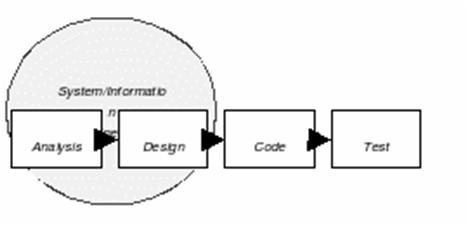
\includegraphics{gambar/analisis}
    \caption{Model pengembangan waterfall.}
    \label{analisis}
\end{figure}

Dengan sistem  web service  diharapkan akan meningkatkan kolaborasi antar pemrogram dan antar organisasi bisnis, yang memungkinkan suatu fungsi dalam web service  dapat digunakan oleh aplikasi lain tanpa perlu mengetahui detil pemrograman yang terdapat di dalamnya. 

Dalam perkembangannya, model  web service  memiliki dua metode yang berorientasi pada layanan dan sumberdaya informasi, yaitu: SOAP dan REST dan yang akan digunakan adalah metode SOAP. 
SOAP (Simple Object Access Protocol) merupakan protokol yang digunakan untuk mempertukarkan data atau informasi dalam format XML (Scheinblum, 2001). SOAP dapat dikatakan sebagai gabungan antara HTTP dengan XML karena SOAP umumnya menggunakan protokol HTTP sebagai sarana transport datanya dan data yang akan dipertukarkan ditulis dalam  format  XML.  Karena  SOAP  menggunakan  HTTP  dan  XML  maka  SOAP  memungkinkan  pihak-pihak  yang mempunyai platform, sistem operasi dan perangkat lunak yang berbeda dapat saling mempertukarkan datanya. 

\subsection{Identifikasi Kebutuhan Sistem}
Analisa sistem yang sedang berjalan pada sebuah sistem pembelajaran elearning Universitas Muhammadiyah Jember menunjukkan bahwasanya dalam akses elearning distribusi data yang ditampilkan dalam sistem informasi elearning diambil langsung dari database server pusat. 

Universitas merupakan sistem yang kompleks yang terdiri dari banyak fakultas, jurusan, dan bagian-bagian yang lain dan banyaknya jumlah mahasiswa. Karena lingkup universitas yang besar, maka penerapan sistem informasi yang terpusat akan terlalu membebani server pusat. Kurang teroganisasinya sistem informasi dapat memperlambat penyampaian informasi sehingga mengganggu jalannya kegiatan  perkuliahan. Salah satu cara dalam mengoptimalkan kinerja sistem informasi adalah dengan merelasikan data yang diperlukan, yang bersumber dari berbagai integrasi aplikasi yang ada. Hal tersebut merupakan sistem kerja dari web service.

\begin{figure}[ht!]
  \centering
    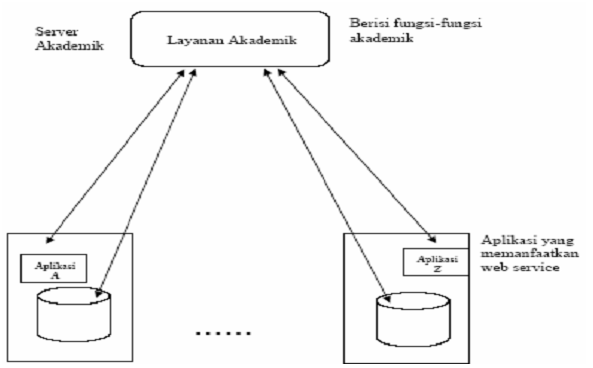
\includegraphics{gambar/server}
    \caption{Gambaran Umum Layanan Informasi Akademik.}
    \label{server}
\end{figure}

Dalam perancangan sistem berbasis  XML  Web Services untuk sistem informasi elearning universitas berikut disajikan langkah-langkah yang perlu dilakukan:

\vspace{-0.5cm}

\begin{enumerate}[a.]
\begin{singlespace}
\itemsep0em
\item Pendefinisian fungsi-fungsi yang akan digunakan dalam sistem informasi elearning universitas.
\item Pengkategorian fungsi-fungsi tersebut. 
\item Pengkodean Web Service.
\item Pengujian fungsi. 
\end{singlespace}
\end{enumerate}

Web  Service  layanan  akademik  yang  dibuat  diletakkan  pada  server.   Aplikasi client  berkomunikasi  dengan  layanan  akademik  dengan cara  memanggil fungsi yang  tersedia  pada   Web Services sambil  mengirimkan  parameter-parameter yang  dibutuhkan.  Pemrosesan  data  dalam  hal  ini  dilakukan  di  server,  kemudian hasil yang diperoleh dikirimkan kembali ke aplikasi client.  

Yang perlu dilakukan terlebih dahulu adalah membuat semua fungsi-fungsi (berupa Web method) yang dapat digunakan untuk mengakses dan mengolah data.  Web method-Web method tersebut diuji fungsionalitasnya, apakah sudah sesuai dengan yang diinginkan. Langkah berikutnya adalah membuat aplikasi client yang nantinya dapat mengakses Web Service  tersebut.
Fasilitas atau fungsi-fungsi yang seringkali dibutuhkan oleh pengembang aplikasi adalah sebagai berikut: 
\vspace{-0.5cm}

\begin{enumerate}[a.]
\begin{singlespace}
\itemsep0em
\item Fungsi-fungsi penambahan, penghapusan, dan pengeditan data.
\item Fungsi-fungsi untuk menampilkan data berdasar kriteria tertentu.
\item Fungsi-fungsi untuk pengolahan data. 
\item Fungsi-fungsi untuk pencarian data berdasar kriteria tertentu.
\end{singlespace}
\end{enumerate}

\subsection{Rancangan basis data}
Untuk rancangan web service elearning diperlukan 5 database
\vspace{-0.5cm}

\begin{enumerate}[1.]
\begin{singlespace}
\itemsep0em
\item Tabel Mahasiswa
\item Tabel Dosen
\item Tabel Mata Kuliah
\item Tabel Fakultas
\item Tabel Jurusan
\end{singlespace}
\end{enumerate}

Berdasar rancangan layangan akademik maka dapat dibuat daftar Web method-Web method yang akan diimplementasikan sebagai berikut: 

\vspace{-0.5cm} 

\begin{enumerate}[1.]
\begin{singlespace}
\itemsep0em
\item Web method  dengan kegunaan penambahan, penghapusan, dan pengeditan data
\end{singlespace}
\end{enumerate}

\vspace{-0.5cm}

\begin{enumerate}[a.]
\begin{singlespace}
\itemsep0em
\item Tambah data mahasiswa. 
\item Tambah data dosen. 
\item Tambah data jadwal kuliah. 
\item Edit data mahasiswa.
\end{singlespace}
\end{enumerate}

\vspace{-0.5cm}

\begin{enumerate}[2.]
\begin{singlespace}
\itemsep0em
\item Web method  dengan kegunaan menampilkan data. 
\end{singlespace}
\end{enumerate}

\vspace{-0.5cm}

\begin{enumerate}[a.]
\begin{singlespace}
\itemsep0em
\item Tampil mata kuliah berdasar kriteria tertentu. 
\item Tampil data dosen berdasar kriteria tertentu.  
\item Tampil data mahasiswa berdasar kriteria tertentu.
\end{singlespace}
\end{enumerate}

\vspace{-0.5cm}

\begin{enumerate}[3.]
\begin{singlespace}
\itemsep0em
\item Web method  dengan kegunaan pencarian data.  
\end{singlespace}
\end{enumerate}

\vspace{-0.5cm}
\begin{enumerate}[a.]
\begin{singlespace}
\itemsep0em
\item Pencarian mata kuliah berdasar kriteria tertentu . 
\item Pencarian data mahasiswa berdasar kriteria tertentu .  
\item Pencarian data dosen berdasar kriteria tertentu.
\end{singlespace}
\end{enumerate}


\section{Jadwal Kegiatan}
Penelitian direncanakan akan dilaksanakan selama enam bulan. Rincian rencana jadwal penelitian dicantumkan dalam tabel berikut.

\begin{center}
Tabel 3.1. Jadwal Penelitian.
\end{center}
\vspace{-0.5cm}
\begin{figure}[ht!]
  \centering
    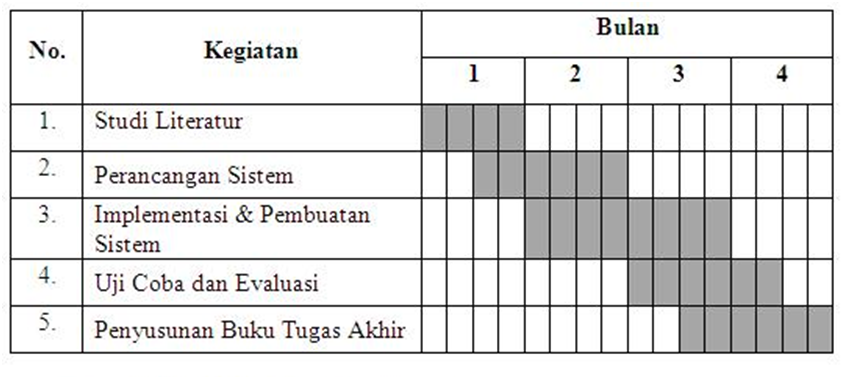
\includegraphics[width=13cm]{gambar/timeline}
\end{figure}

%-----------------------------------------------------------------
%Disini akhir masukan Bab
%-----------------------------------------------------------------

%-----------------------------------------------------------------
%Disini awal masukan untuk Daftar Pustaka
%-----------------------------------------------------------------
%%\nocite{Abel2010,Guerbas201350}
%%\bibliography{research-plan}
%%\bibliographystyle{plainnat}
\begin{thebibliography}{9}

\bibitem[satu(2013)]{satu01}
Chaudary, A.S,  Saleem,  M.A,  Bukhary,  H.Z. (2003).  Web  Services  and Distributed Applications. Advantages and  Problems .  Internet Resources.

\bibitem[dua(2013)]{dua02}
E. Christensen, F. Curbera,  G. Meredith, S. Weerawarana:  Web Services Description Language.

\bibitem[tiga(2013)]{tiga03}
(WSDL) 1.1 , 15 March 2001.http://www.w3.org/TR/wsdl.

\bibitem[empat(2013)]{empat04}
Kamil, M.(2010).e-Learning Sebuah Prospek Pembelajaran.

\end{thebibliography}
\addcontentsline{toc}{chapter}{DAFTAR PUSTAKA}
%-----------------------------------------------------------------
%Disini akhir masukan Daftar Pustaka
%-----------------------------------------------------------------

\end{document}
